%%%%%%%%%%%%%%%%%%%%%%%%%%%%%%%%%%%%%%%%%%%%%%%%%%%%%%%%%%%%%%%%%%%%%%%%%%%%%%%
% Chapter 'Absorption - R-143a - lubricant PEC9'
%%%%%%%%%%%%%%%%%%%%%%%%%%%%%%%%%%%%%%%%%%%%%%%%%%%%%%%%%%%%%%%%%%%%%%%%%%%%%%%
\subsection{Lubricant PEC9}
%
%%%%%%%%%%%%%%%%%%%%%%%%%%%%%%%%%%%%%%%%%%%%%%%%%%%%%%%%%%%%%%%%%%%%%%%%%%%%%%%
%%%%%%%%%%%%%%%%%%%%%%%%%%%%%%%%%%%%%%%%%%%%%%%%%%%%%%%%%%%%%%%%%%%%%%%%%%%%%%%
\subsubsection{FloryHuggins - ID 1}
%
\begin{tabular}[l]{|lp{11.5cm}|}
\hline
\addlinespace

\textbf{Sorbent:} & lubricant \\
\textbf{Subtype:} & PEC9 \\
\textbf{Refrigerant:} & R-143a \\
\textbf{Equation:} & FloryHuggins \\
\textbf{ID:} & 1 \\
\textbf{Reference:} & Wahlström, Åsa; Vamling, Lennart (2000): Solubility of HFCs in Pentaerythritol Tetraalkyl Esters. In: J. Chem. Eng. Data 45 (1), S. 97–103. DOI: 10.1021/je990171n. \\
\textbf{Comment:} & None \\

\addlinespace
\hline
\end{tabular}
\newline

\textbf{Equation and parameters:}
\newline
%
Pressure $p$ in $\si{\pascal}$ is calculated depending on molar fraction of refrigerant in the liquid phase $x_1$ in $\si{\mole\per\mole}$, temperature $T$ in $\si{\kelvin}$, molar volumes of both components ($v_1$ and $v_2$) in $\si{\cubic\meter\per\mole}$, and vapor pressure $p_\mathrm{sat,1}$ in $\si{\pascal}$. If molar volumes less than zero are used as function arguements, constant molar volumes given by parameter record are used. Equilibrium equation is given by:
%
\begin{equation*}
\begin{split}
p &=& \gamma_1 x_1 p_\mathrm{sat,1} & \quad\text{, and} \\
\gamma_1 &=& \exp \left( \ln \left( 1 - \left( 1 - \nicefrac{1}{r} \right) \Phi_2  \right) + \left(1 - \nicefrac{1}{r}\right) \Phi_2 + \Gamma \Phi_2 ^2 \right) & \quad\text{, and} \\
\Phi_2 &=& r \frac{x_2}{x_1 + r x_2} & \quad\text{, and} \\
\Gamma &=& \nicefrac{w_0^{*}}{T} \left( 1 + \nicefrac{w_1}{T} \right) & \quad\text{, and} \\
x_2 &=& 1 - x_1  & \quad\text{.} \\
\end{split}
\end{equation*}
%
The parameters of the equation are:
%
\begin{longtable}[l]{lll|lll}
\toprule
\addlinespace
\textbf{Par.} & \textbf{Unit} & \textbf{Value} &	\textbf{Par.} & \textbf{Unit} & \textbf{Value} \\
\addlinespace
\midrule
\endhead

\bottomrule
\endfoot
\bottomrule
\endlastfoot
\addlinespace

$r$ & - & 7.790000000e+00 & $w_0^{*}$ & $\si{\kelvin}$ & 8.170000000e+02 \\
$w_1$ & $\si{\kelvin}$ & -1.520000000e+02 & & & \\

\addlinespace\end{longtable}

\textbf{Validity:}
\newline
Equation is approximately valid for $303.15 \si{\kelvin} \leq T \leq 363.15 \si{\kelvin}$.
\newline

\textbf{Visualization:}
%
\begin{figure}[!htp]
{\noindent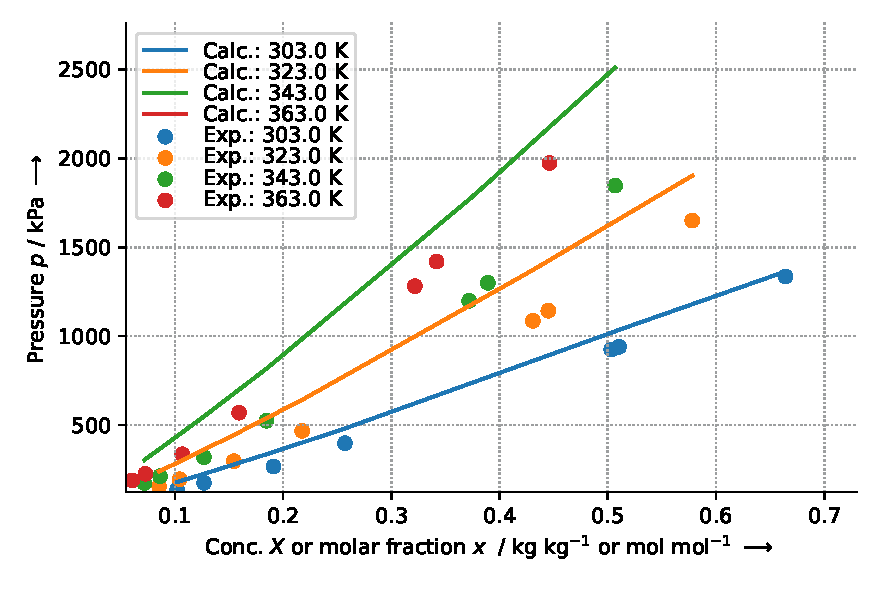
\includegraphics[height=10cm, keepaspectratio]{figs/abs/abs_R-143a_lubricant_PEC9_FloryHuggins_1.pdf}}
\end{figure}
%

To generate the figure, the following refrigerant functions were selected:
\begin{itemize}
\item Vapor pressure: VaporPressure\_EoS1 - ID 1
\item Saturated liquid density: SaturatedLiquidDensity\_EoS1 - ID 1
\end{itemize}

The uncertainity of the experimental data is:
\begin{itemize}
\item Data source $\,\to\,$ Data was taken from table
\end{itemize}

The mean absolute percentage error (MAPE) between the experimental and calculated data results in 37.87\%.
\FloatBarrier
\newpage
%%%%%%%%%%%%%%%%%%%%%%%%%%%%%%%%%%%%%%%%%%%%%%%%%%%%%%%%%%%%%%%%%%%%%%%%%%%%%%%
